
\todo{There should be a link either here or at end of literature which forms the basic for different methods (clustering, routing, trip generation).}
\todo{Paragraph describing different types of algorithm used (Routing then cluster, Cluster then Routing, Genetic, etc.)}
\todo{Remember to justify the choice of algorithms. You may also need to explain how to adopt these algorithms in your work. A figure showing the ralationship between different components of your work may also help.}
\subsection{Routing}\label{subsec:routing}
\todo{Explain purpose of routing/goal of algorithms.}
\subsubsection{Brute Force}\label{subsubsec:brute-force-routing}
\todo{Write brute force explanation}
The brute force algorithm is a simple one that simply tries every possible route and returns the best one.
It is guaranteed to find the optimal route, however it's computational cost becomes impractical as input size grows,
with a time complexity of $O(n!)$.
Considering we will be comparing algorithms based on their speed and the quality of their results, brute force is a
useful benchmark, providing a lower bound for speed and an upper bound for quality.
\pagebreak
For a given input the number of days $d$ and the number of locations $n$ will be used to form a set that contains
'0' $d-1$ times and the numbers from '1' to $n$ once.
\begin{equation}
    Set Builder(n,d) = {\{0^{\times d-1}, 1, 2, ..., n-1\}}
\end{equation}
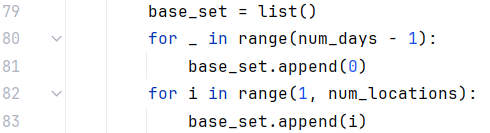
\includegraphics[width=0.75\textwidth]{Brute_force_set_generation}
\subsubsection{Greedy Routing/Insertion}\label{subsubsec:greedy-routing}
\todo{Explain greedy routing algorithm}
\todo{Explain greedy insertion algorithm}
\subsubsection{Gift Wrapping}\label{subsubsec:gift-wrapping}
\todo{Explain gift wrapping algorithm}
\todo{Something like: "Once gift wrapping has found a convex hull, a greedy insertion algorithm is used to find the optimal route within the convex hull."}

\subsection{Clustering}\label{subsec:clustering}
\todo{Explain purpose of clustering, how it is used in route planning and the goal of our algorithms.}
\subsubsection{K-Means}\label{subsubsec:k-means}
\todo{Explain k-means algorithm}

\subsection{Trip Generation}\label{subsec:trip-generation}
\todo{Explain trip generation, how it is used in route planning and the goal of our algorithms.}
\subsubsection{Brute Force}\label{subsubsec:brute-force-trip-generation}
\todo{Explain how brute force algorithm can be modified for trip generation.}

\subsection{Genetic Algorithms}\label{subsec:genetic-algorithm}
\todo{Explain basics of genetic algorithms, include how by considering different genomes, the algorithm can be used for routing, clustering or trip generation.}
\subsubsection{General Clustering}
\todo{Explain genetic clustering}
\subsubsection{Centroid-based Clustering}
\todo{Explain genetic centroid-based clustering and how it differs from general clustering.}
\subsubsection{Routing}
\todo{Explain genetic routing}
\subsubsection{Trip Generation}
\todo{Explain genetic trip generation}